\documentclass[submit]{harvardml}

\newboolean{solutionCopy}
\setboolean{solutionCopy}{true} % Toggle between solution copy and distro

\ifthenelse{\boolean{solutionCopy}}{
  \includeversion{solution}
}{
  \excludeversion{solution}
}

% Put in your full name and email address.
\name{Shawn Pan}
\email{shawn\_pan@g.harvard.edu}

% List any people you worked with.
\collaborators{%
  Chin Hui Chew
}

% You don't need to change these.
\course{CS181-S17}
\assignment{Assignment \#2}
\duedate{5:00pm Feb 24th, 2017}

\usepackage[OT1]{fontenc}
\usepackage[colorlinks,citecolor=blue,urlcolor=blue]{hyperref}
\usepackage[pdftex]{graphicx}
\usepackage{subfig}
\usepackage{fullpage}
\usepackage{amsmath}
\usepackage{amssymb}
\usepackage{color}
\usepackage{todonotes}
\usepackage{listings}
\usepackage{common}
\usepackage{bm}

\usepackage[mmddyyyy,hhmmss]{datetime}

\definecolor{verbgray}{gray}{0.9}

\lstnewenvironment{csv}{%
  \lstset{backgroundcolor=\color{verbgray},
  frame=single,
  framerule=0pt,
  basicstyle=\ttfamily,
  columns=fullflexible}}{}

\begin{document}


%%% Change the assignment details here:

\ifthenelse{\boolean{solutionCopy}}{
\begin{center}
{\Large \textbf{SOLUTION - Do Not Distribute}\\Homework 2: Bayesian Methods and Multiclass Classification}\\
\end{center}
}{
  \begin{center}
{\Large Homework 2: Bayesian Methods and Multiclass Classification}\\
\end{center}
}
\subsection*{Introduction}

This homework is about Bayesian methods
and  multiclass classification. In lecture we have
primarily focused on binary classifiers trained to discriminate
between two classes. In multiclass classification, we discriminate
between three or more classes. We encourage you to first read the
Bishop textbook coverage of these topic, particularly: Section 4.2
(Probabilistic Generative Models), Section 4.3 (Probabilistic
Discriminative Models).
%, and, if MLE is troublesome, review
%the materal Section 1
%and lecture 3.

As usual, we imagine that we have the input matrix $\boldX \in
\reals^{n \times m}$ (or perhaps they have been mapped to some basis
$\bm{\Phi}$, without loss of generality) but our outputs are now
``one-hot coded''.  What that means is that, if there are~$c$ output
classes, then rather than representing the output label $y$ as an
integer~${1,2,\ldots,c}$, we represent $\boldy$ as a binary vector of
length~$c$. These vectors are zero in each
component except for the one corresponding to the correct label, and
that entry has a one.  So, if there are 7 classes and a particular
datum has label 3, then the target vector would be~${C_3 = [0,0,1,0,0,0,0]}$.
If there are $c$ classes, the set of possible outputs is $\{C_1 \ldots C_c \} = \{C_k\}_{k=1}^c$.
Throughout the assignment we will assume
that output $\boldy \in \{C_k\}_{k=1}^c$.\\

The problem set has four problems:
\begin{itemize}
\item In the first problem, you will explore the properties of Bayesian
estimation methods for the Bernoulli model as well as the special
case of Bayesian linear regression with a simple prior.
%
\item In the second problem, you will explore the properties of the softmax
function, which is central to
the method of
multiclass logistic regression.
%We will also see that the
%softmax plays a key role in  neural networks.
%
\item  In the third
problem, you will dive into  matrix algebra and the methods behind
generative multiclass classifications. You will extend the discrete classifiers
that we see in  lecture to a Gaussian model.
%
\item Finally, in the fourth problem, you will implement
 logistic regression as well as a generative classifier
from close to scratch.
%
\end{itemize}

\newpage
\begin{problem}[Bayesian Methods, 10 pts]

  This question helps to build your understanding of the
  maximum-likelihood estimation (MLE) vs. maximum a posterior estimator
  (MAP) and posterior predictive estimator, first in the
  Beta-Bernoulli model and then in the linear regression setting.\\

First consider the Beta-Bernoulli model (and see lecture 5.)
%
\begin{enumerate}
\item[1.] Write down the expressions for the MLE, MAP and posterior predictive
distributions, and for
a prior $\theta\sim Beta(4,2)$ on the
parameter of the Bernoulli,
and  with data $D= 0, 0, 1, 1, 0, 0, 0, 0, 1, 0, 1, 1,$
$1, 0, 1, 0$, plot
the three different
estimates after each additional
sample.
%
\item[2.] Plot the posterior distribution (prior for 0 examples) on $\theta$ after 0, 4, 8, 12 and 16
examples. (Using whatever tools you like.)
%
\item[3.] Interpret the differences you see between the three different
estimators.
%
%note, initial skew is to large 1, but data has $\theta=0.4$
%
\end{enumerate}

Second, consider the Bayesian Linear Regression model, with
data $D=\{(\boldx_i,y_i)\}_{i=1}^n$, $\boldx_i\in\mathbb{R}^m$,
 $y_i\in\mathbb{R}$, and generative model
%
$$
y_i\sim\mcN(\boldw^\top\boldx_i,\beta^{-1})
$$
for (known) precision $\beta$ (which is just the reciprocal
of the variance). Given this, the likelihood of the
data is $p(\boldy|\boldX,\boldw) = \mcN(\boldy|\boldX\boldw,\beta^{-1}\mathbf{I})$. Consider the special case of
an isotropic (spherical) prior on weights, with
%
$$
p(\boldw)=\mcN(\boldw|\bold0,\alpha^{-1}\boldI)
$$

\begin{enumerate}
\item[4.] Justify when you might use this prior in practice.
%
\item[5.] Using the method in lecture of taking logs, expanding and pushing terms
that don't depend on $\boldw$ into a constant, and finally collecting
terms and completing the square, confirm that the posterior on
weights after data $D$ is $\boldw\sim\mcN(\boldw|\boldm_n,\boldS_n)$,
where
%
\begin{align*}
\boldS_n&=(\alpha\boldI+\beta\boldX^\top\boldX)^{-1}\\
\boldm_n&=\beta\boldS_n\boldX^\top\boldy
\end{align*}
\item[6.] Derive the special case
of the MAP estimator for this problem as the isotropic
prior becomes arbitrarily weak.
What does the MAP estimator reduce to?
%
\item[7.] What did we observe in lecture about this
estimator for the case where
the prior is neither weak nor strong?
\end{enumerate}
\end{problem}

\begin{solution}
\begin{sol}
\begin{enumerate}
\item Let $n_0$ be the number of $0$s in the data and $n_1$ be the number of $1$s.
As derived from the lecture 5 slides:
\begin{align*}
\theta_{\textrm{MLE}} &= \frac{n_1}{n_0 + n_1}\\
\theta_{\textrm{MAP}} &= \frac{\alpha + n_1 - 1}{\alpha + \beta + n_0 + n_1 - 2}\\
&= \frac{3 + n_1}{4 + n_0 + n_1}\\
p(x=1 \given D) &= \frac{\alpha + n_1}{\alpha + \beta + n_1 + n_0}\\
&= \frac{4 + n_1}{6 + n_0 + n_1}
\end{align*}

\begin{figure}[h!]
  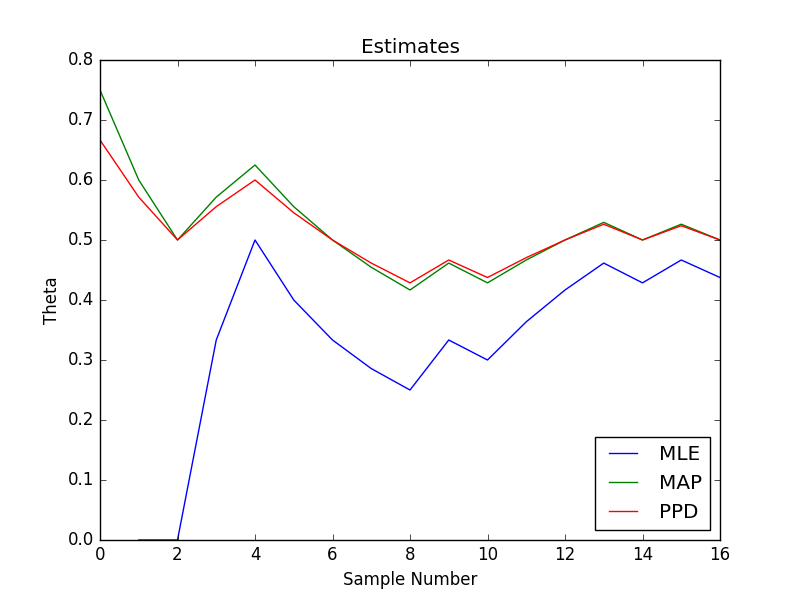
\includegraphics[width=4.5in]{problem1part1.png}
  \caption{Problem 1.1}
\end{figure}
%
\item See plot.
\begin{figure}[h!]
  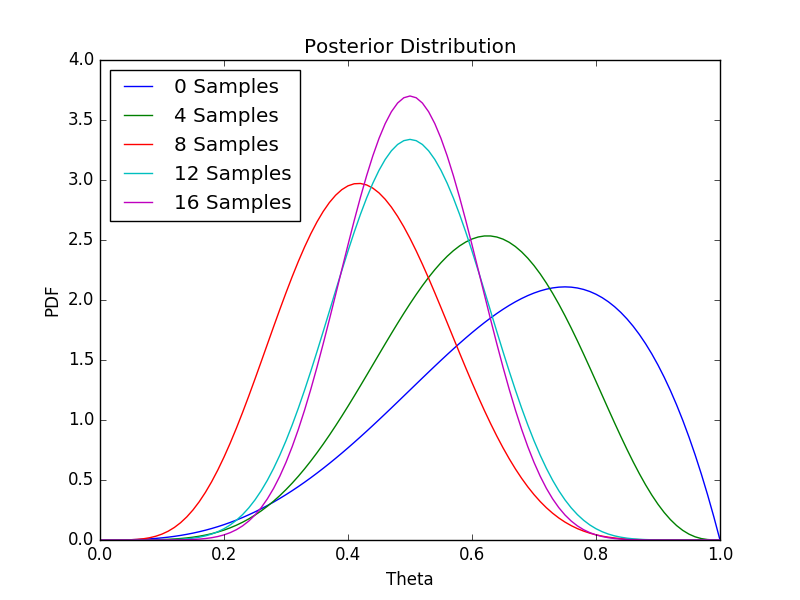
\includegraphics[width=4.5in]{problem1part2.png}
  \caption{Problem 1.2}
\end{figure}
%
\item
The graph for MLE is lower than that of the MAP and PPD, because the MLE does not take the prior into account and the first two data points are 0.
As more data points are added, the prior has less importance and the estimates approach each other.
The MAP represents the mode of the posterior distribution, while the PPD represents the expected value.
The MAP and PPD are very similar, other than the MAP being slightly further from 0.5 than the PPD, due to the distributions having a longer tail on one side.
%
\item
You may want to use a isotropic zero-centered normal prior on weights for regularization.
You want your linear regression model to have small magnitude weights to have lower variance, and adding a prior gives a preference for smaller magnitude weights.
%
\item
\begin{align*}
p(\boldw | \boldX) &\propto p(\boldy | \boldX, \boldw) p(\boldw)\\
\ln p(\boldw | \boldX) &\propto \ln p(\boldy | \boldX, \boldw) + \ln p(\boldw)\\
&= -\frac12 (\boldy - \boldX\boldw)^T (\beta \boldI) (\boldy - \boldX\boldw) -\frac12(\boldw - \bold0)^T (\alpha \boldI) (\boldw - \bold0) + \textrm{const}\\
&= -\frac12 (\beta \boldy^T \boldy - \beta \boldy^T \boldX \boldw - \beta \boldw^T \boldX^T \boldy + \beta \boldw^T \boldX^T \boldX \boldw + \alpha \boldw^T \boldw) + \textrm{const}\\
&= -\frac12 \left(- \beta \boldy^T \boldX \boldw - \beta \boldw^T \boldX^T \boldy + \boldw^T (\beta \boldX^T \boldX + \alpha \boldI) \boldw \right) + \textrm{const}
\end{align*}
We now expand out $\ln p(\boldw | \boldX)$, so we can match terms to complete the square.
\begin{align*}
\ln p(\boldw | \boldX) &= -\frac12 (\boldw - \boldm_n)^T \boldS_n^{-1} (\boldw - \boldm_n) + \textrm{const} \\
&= \boldw^T \boldS_n^{-1} \boldw - \boldw^T \boldS_n^{-1} \boldm_n - \boldm_n^T \boldS_n^{-1} \boldw + \textrm{const}
\end{align*}
Matching terms, we have the following.
\begin{align*}
\boldS_n^{-1} &= \beta \boldX^T \boldX + \alpha \boldI\\
\boldS_n &= (\beta \boldX^T \boldX + \alpha \boldI)^{-1}\\
\boldS_n^{-1} \boldm_n &= \beta \boldX^T \boldy\\
\boldm_n &= \beta \boldS_n^{-1} \boldX^T \boldy
\end{align*}
%
\item
With $\alpha = 0$ we have $\boldS_n = (\beta\boldX^\top\boldX)^{-1}$ and
$\boldm_n =\beta(\beta\boldX^\top\boldX)^{-1}\boldX^\top\boldy = (\boldX^\top\boldX)^{-1}\boldX^\top\boldy$
which is equivalent to ordinary least squares regression.
%
\item
Linear regression with a normal prior is equivalent to ridge regression.
When the prior is a balance between weak and strong, the regularization effect because a tradeoff between bias and variance.
With cross-validation, one can find a good prior for the model.


\end{enumerate}
\end{sol}
\end{solution}


\newpage
%\subsection*{1. Properties of Softmax [5pts]}
%%%%%%%%%%%%%%%%%%%%%%%%%%%%%%%%%%%%%%%%%%%%%
% Problem 1
%%%%%%%%%%%%%%%%%%%%%%%%%%%%%%%%%%%%%%%%%%%%%
\begin{problem}[Properties of Softmax, 8pts]
%
  We have explored logistic regression, which is a discriminative
  probabilistic model over two classes. For each input $\boldx$,
  logistic regression outputs a probability of the class output $y$
  using the logistic sigmoid function.

  The softmax transformation is an important generalization of the logistic
  sigmoid to the case of $c$ classes. It takes as input a vector, and
  outputs a transformed vector of the same size,
%
  \[ \mathrm{softmax}(\boldz)_k =\frac{\exp(z_k)}{\sum_{\ell=1}^c \exp(z_{\ell})}, \ \ \text{for all $k$}\]

Multiclass logistic regression uses the softmax transformation over vectors of size $c$. Let $\{\boldw_{\ell}\} = \{\boldw_1 \ldots \boldw_c \} $
denote the parameter vectors for each class.
In particular,  multiclass logistic regression
defines the probability of class $k$ as,
%
\begin{align*}
  p(\boldy=C_k \given \boldx; \{\boldw_{\ell}\})
  &= \mathrm{softmax}([\boldw_1^{\top}\boldx \ldots \boldw_c^{\top} \boldx]^\top)_k =  \frac{ \exp( \boldw_k^{\top}\boldx ) }
  {  \sum_{\ell=1}^c \exp( \boldw_{\ell}^{\top}\boldx ) }\,.
\end{align*}

\noindent  As above, we are
using~$\boldy = {C_{k}}$ to indicate the output
vector that represents class $k$.

Assuming data $D = \{(\boldx_i, \boldy_i)\}_{i=1}^n$,
the negated log-likelihood  can be written in the standard form, as
%
\[\mcL(\{\boldw_{\ell}\}) = - \sum_{i=1}^n \ln  p(\boldy_i \given \boldx_i; \{\boldw_{\ell}\}) \]


Softmax is an important function in the context of machine learning,
and you will see it again in other models, such as neural networks.
In this problem, we aim to gain intuitions into the properties of
softmax and multiclass logistic regression.

Show that:
\begin{enumerate}
  \item The output of the softmax function is a vector with non-negative components
    that are at most 1.
%
  \item The output of the softmax function defines a distribution,
so that in addition, the components sum to 1.
%
  \item Softmax preserves order. This means that if elements $z_k < z_\ell$,
in $\boldz$, then  $\mathrm{softmax}(\boldz)_k < \mathrm{softmax}(\boldz)_{\ell}$ for any $k,\ell$.
  \item Show that \[\frac{\partial \mathrm{softmax}(\boldz)_k }{\partial z_j} = \mathrm{softmax}(\boldz)_k (I_{kj} - \mathrm{softmax}(\boldz)_j) \ \ \text{for\ any\ } k, j  \],
%
where indicator $I_{kj}=1$ if $k=j$ and $I_{kj}=0$ otherwise.
%
  \item Using your answer to the previous question, show that
    \[ \frac{\partial }{\partial \boldw_k} \mcL(\{\boldw_{\ell}\}) = \sum_{i=1}^n (p(\boldy_i = C_k | \boldx_i; \{\boldw_\ell\}) - y_{ik} ) \boldx_i  \]
    By the way, this may be useful for Problem 3!
\end{enumerate}
\end{problem}


\begin{solution}
\begin{sol}
\begin{enumerate}
\item Note that $\exp(z) > 0$ for all $z$. Therefore, $\sum_{\ell=1}^c \exp(z_{\ell}) > 0$.
Each component of the output of softmax is therefore a positive number divided by a positive number which is positive.
The denominator is the sum of positive numbers including the term in the numerator, so the denominator is greater than the numerator.
Therefore, each component is also at most 1.
%
\item
\begin{align*}
\sum_{k=1}^{c} {\mathrm{softmax}(\boldz)_k} &= \sum_{k=1}^{c} \frac{\exp(z_k)}{\sum_{\ell=1}^c \exp(z_{\ell})}\\
&= \frac{\sum_{k=1}^{c} \exp(z_k)}{\sum_{\ell=1}^c \exp(z_{\ell})}\\
&= 1
\end{align*}
%
\item
\begin{align*}
z_k &< z_l\\
\exp(z_k) &< \exp(z_l)\\
\frac{\exp(z_k)}{\sum_{m=1}^c \exp(z_{m})} &< \frac{\exp(z_l)}{\sum_{m=1}^c \exp(z_{m})}\\
\mathrm{softmax}(\boldz)_k &< {\mathrm{softmax}(\boldz)_l}
\end{align*}
%
\item
\begin{align*}
\frac{\partial \mathrm{softmax}(\boldz)_k }{\partial z_j} &= \frac{\partial}{\partial z_j} \left( \frac{\exp(z_k)}{\sum_{\ell=1}^c \exp(z_{\ell})} \right)\\
&= \frac{ \left(\sum_{\ell=1}^c \exp(z_{\ell})\right) \frac{\partial}{\partial z_j} \exp(z_k)
- \exp(z_k) \frac{\partial}{\partial z_j} \left( \sum_{\ell=1}^c \exp(z_{\ell}) \right)}
{ \left( \sum_{\ell=1}^c \exp(z_{\ell}) \right)^2}\\
&= \frac{\frac{\partial}{\partial z_j} \exp(z_k)}{\sum_{\ell=1}^c \exp(z_{\ell})}
- \left(\frac{\exp(z_k)}{\sum_{\ell=1}^c \exp(z_{\ell})}\right)
\left(\frac{\exp(z_j)}{\sum_{\ell=1}^c \exp(z_{\ell})}\right)\\
&= \mathrm{softmax}(\boldz)_k I_{kj} - \mathrm{softmax}(\boldz)_k \mathrm{softmax}(\boldz)_j\\
&= \mathrm{softmax}(\boldz)_k (I_{kj} - \mathrm{softmax}(\boldz)_j)
\end{align*}
%
\item
For convenience, we define $S = p(\boldy=C_k \given \boldx; \{\boldw_{\ell}\}) = \mathrm{softmax}([\boldw_1^{\top}\boldx \ldots \boldw_c^{\top} \boldx]^\top)_k$.
\begin{align*}
\frac{\partial }{\partial \boldw_k} \mcL(\{\boldw_{\ell}\}) &= \frac{\partial }{\partial \boldw_k} \left( - \sum_{i=1}^n \sum_{k=1}^c y_{ik} \ln S \right)\\
&= - \sum_{i=1}^n y_{ik} \frac{\partial \ln S}{\partial \boldw_k}\\
&= - \sum_{i=1}^n y_{ik} \frac{\partial \ln S}{\partial S} \frac{\partial S}{\partial \boldw_k^T\boldx_i} \frac{\partial \boldw_k^T\boldx_i}{\partial \boldw_k}\\
&= - \sum_{i=1}^n y_{ik} \frac{1}{S} S(1 - S) \boldx_i\\
&= \sum_{i=1}^n (S - y_{ik}) \boldx_i\\
&= \sum_{i=1}^n (p(\boldy_i = C_k | \boldx_i; \{\boldw_\ell\}) - y_{ik} ) \boldx_i
\end{align*}

\end{enumerate}
\end{sol}
\end{solution}

%\subsection*{2. Mooooar matrix calculus [10 pts]}
%%%%%%%%%%%%%%%%%%%%%%%%%%%%%%%%%%%%%%%%%%%%%
% Problem 2
%%%%%%%%%%%%%%%%%%%%%%%%%%%%%%%%%%%%%%%%%%%%%
\begin{problem}[Return of matrix calculus, 10pts]

  Consider now a generative $c$-class model.  We adopt class prior
  $p(\boldy = C_k; \bpi) = \pi_k$ for all $k \in \{1, \ldots, c\}$
(where $\pi_k$ is a parameter of the prior).
%
%that define the prior.
Let  $p(\boldx|\boldy=C_k)$ denote
the class-conditional density of features $\boldx$ (in this
case for class $C_k$). Consider the data set $D = \{(\boldx_i,
\boldy_i)\}_{i=1}^n$ where as above $\boldy_i \in \{C_k\}_{k=1}^c$ is
encoded as a one-hot target vector.
%
\begin{enumerate}
  \item Write out the negated log-likelihood of the data set,
    $-\ln p(D ; \bpi)$.
%
  \item Since the prior forms a distribution, it has the constraint that
    $\sum_k\pi_k - 1 = 0$.  Using the hint on
Lagrange multipliers below, give the
    expression for the maximum-likelihood estimator for the prior
    class-membership probabilities, i.e.
    $\hat \pi_k.$
    Make sure to write out the intermediary equation you need
    to solve to obtain this estimator. Double-check your answer: the final
    result should be very intuitive!
\end{enumerate}

    For the remaining questions, let the
    class-conditional probabilities be Gaussian distributions with
the same covariance matrix
    $$p(\boldx | \boldy = C_k) = \mathcal{N}(\boldx |  \bmu_k, \bSigma), \text{\ for\ }k \in \{1,\ldots, c\}$$
%
and different means $\bmu_k$ for each class.
%
    \begin{enumerate}
  \item[3.] Derive the gradient of the negative log-likelihood with respect to vector $\bmu_k$.
    Write the expression in matrix form as a function of the variables defined
    throughout this exercise. Simplify as much as possible for full credit.
  \item[4.] Derive the maximum-likelihood estimator for vector $\bmu_k$. Once
    again, your final answer should seem intuitive.
  \item[5.] Derive the gradient for the negative log-likelihood with respect to the
    covariance matrix $\bSigma$ (i.e., looking
to find an MLE for the covariance).
Since you are differentiating with respect to a
    \emph{matrix}, the resulting expression should be a matrix!
%
  \item[6.] Derive the maximum likelihood estimator of the covariance matrix.
\end{enumerate}

\paragraph{[Hint: Lagrange Multipliers.} Lagrange Multipliers are a method for
optimizing a function $f$ with respect to an
equality constraint, i.e.
\[\min_{\boldx} f(\boldx)\ \text{s.t.}\ g(\boldx) = 0.\]

This can be turned into an unconstrained problem by introducing a
Lagrange multiplier $\lambda$ and constructing the Lagrangian function,
\[L(\boldx, \lambda) =  f(\boldx) + \lambda g(\boldx).\]

It can be shown that it is a necessary condition that the optimum
is a critical point of this new function. We can find this point by solving two equations:

\[\frac{\partial L(\boldx, \lambda)}{\partial  \boldx} = 0  \ \ \text{and}\  \  \frac{\partial L(\boldx, \lambda)}{\partial \lambda} = 0 \]


\paragraph{Cookbook formulas.} Here are some formulas you might want to consider
using to compute difficult gradients. You can use them  in the homework
without proof. If you are looking to hone your matrix calculus skills, try to
find different ways to prove these formulas yourself (will not be part of the
evaluation of this homework). In general, you can use any formula from the matrix cookbook,
as long as you cite it. We opt for the following common notation:
$\boldX^{-\top} := (\boldX^{\top})^{-1}$
\begin{align*}
  & \frac{\partial \bolda^\top \boldX^{-1} \boldb}{\partial \boldX} = - \boldX^{-\top} \bolda \boldb^\top \boldX^{-\top} \\
  & \frac{\partial \ln | \det (\boldX) |}{\partial \boldX} = \boldX^{-\top}
 \end{align*}
 \end{problem}


\begin{solution}
\begin{sol}
\begin{enumerate}
\item
\begin{align*}
-\ln p(D ; \bpi) &= -\ln \prod_{i=1}^n p(\boldx_i | \boldy_i ; \bpi)\\
&= -\ln \prod_{i=1}^n \sum_{k=1}^c y_{ik} p(\boldx_i | \boldy_i = C_k) p(\boldy_i = C_k; \bpi)\\
&= - \sum_{i=1}^n \ln \sum_{k=1}^c y_{ik} p(\boldx_i | \boldy_i = C_k) p(\boldy_i = C_k; \bpi)\\
&= - \sum_{i=1}^n \sum_{k=1}^c y_{ik} \ln p(\boldx_i | \boldy_i = C_k) p(\boldy_i = C_k; \bpi)
\end{align*}
Note that the $\sum_{k=1}^c y_{ik}$ term selects the correct class corresponding to $y_i$.
The last step is valid, because $y_i$ is a one-hot encoded vector and exactly one element in the sum in non-zero.
\begin{align*}
&= - \sum_{i=1}^n \sum_{k=1}^c y_{ik} \ln p(\boldx_i | \boldy_i = C_k)
- \sum_{i=1}^n \sum_{k=1}^c y_{ik} \ln p(\boldy_i = C_k; \bpi)\\
&= - \sum_{i=1}^n \sum_{k=1}^c y_{ik} \ln p(\boldx_i | \boldy_i = C_k)
- \sum_{i=1}^n \sum_{k=1}^c y_{ik} \ln \pi_k
\end{align*}
%
\item
\begin{align*}
L(\bpi, \lambda) &= - \sum_{i=1}^n \sum_{k=1}^c y_{ik} \ln p(\boldx_i | \boldy_i = C_k)
- \sum_{i=1}^n \sum_{k=1}^c y_{ik} \ln \pi_k
+ \lambda \left( \sum_{k=1}^c \pi_k - 1 \right)\\
\frac{\partial L}{\partial \lambda} = 0 &= \sum_{k=1}^c \pi_k - 1\\
\sum_{k=1}^c \pi_k &= 1\\
\frac{\partial L}{\partial \pi_k} = 0 &= - \frac{\sum_{i=1}^n y_{ik}}{\pi_k} + \lambda\\
\pi_k &= \frac{\sum_{i=1}^n y_{ik}}{\lambda}\\
\sum_{k=1}^c \pi_k = 1 &= \frac{\sum_{i=1}^n \sum_{k=1}^c y_{ik}}{\lambda}\\
1 &= \frac{\sum_{i=1}^n 1}{\lambda}\\
\lambda &= n\\
\hat{\pi_k} &= \frac{\sum_{i=1}^n y_{ik}}{n}
\end{align*}
This answer makes sense, because it is simply the fraction of $\boldy$ of a particular class observed in the data.
%
\item
For convenience, we lump off terms that are constant with respect to $\bmu_k$.
Note that because the covariance matrix is symmetric, $\bSigma = \bSigma^T$.
\begin{align*}
\frac{\partial L}{\partial \bmu_k} &=
\frac{\partial}{\partial \bmu_k}\left(
- \sum_{i=1}^n \sum_{k=1}^c y_{ik} \ln \mathcal{N}(\boldx_i |  \bmu_k, \bSigma)
+ \textrm{const}_{\bmu_k}\right)\\
&= \frac{\partial}{\partial \bmu_k}\left(
- \sum_{i=1}^n y_{ik} \left(-\frac12 (\boldx_i-\bmu_k)^T \bSigma^{-1} (\boldx_i-\bmu_k) \right)
+ \textrm{const}_{\bmu_k}\right)\\
&= - \sum_{i=1}^n y_{ik} \left(-\frac12 (\bSigma^{-1} + \bSigma^{-T}) (\boldx_i-\bmu_k) (-1) \right)\\
&= - \sum_{i=1}^n y_{ik} \bSigma^{-1} (\boldx_i-\bmu_k)
\end{align*}
%
\item
We find the MLE by setting the gradient to 0.
\begin{align*}
0 &= - \sum_{i=1}^n y_{ik} \bSigma^{-1} (\boldx_i-\bmu_k)\\
\sum_{i=1}^n y_{ik} \boldx_i &= \sum_{i=1}^n y_{ik} \bmu_k\\
\hat{\bmu_k} &= \frac{\sum_{i=1}^n y_{ik} \boldx_i}{\sum_{i=1}^n y_{ik}}
\end{align*}
This answer makes sense, because it is the mean $\boldx$ among the data points of the given class.
%
\item
For convenience, we lump off terms that are constant with respect to $\bSigma$.
Note that because the covariance matrix is symmetric, $\bSigma = \bSigma^T$.
\begin{align*}
\frac{\partial L}{\partial \bSigma} &=
\frac{\partial}{\partial \bSigma}\left(
- \sum_{i=1}^n \sum_{k=1}^c y_{ik} \ln \mathcal{N}(\boldx_i |  \bmu_k, \bSigma)
+ \textrm{const}_{\bSigma}\right)\\
&= \frac{\partial}{\partial \bSigma}\left(
- \sum_{i=1}^n \sum_{k=1}^c y_{ik} \left(-\frac12 \ln |\bSigma| -\frac12 (\boldx_i-\bmu_k)^T \bSigma^{-1} (\boldx_i-\bmu_k) \right)
+ \textrm{const}_{\bSigma}\right)\\
&= \frac12 \sum_{i=1}^n \sum_{k=1}^c y_{ik}
\left( \bSigma^{-T} - \bSigma^{-T} (\boldx_i-\bmu_k) (\boldx_i-\bmu_k)^T \bSigma^{-T}\right)\\
&= \frac12 \sum_{i=1}^n \sum_{k=1}^c y_{ik}
\bSigma^{-T} \left(I - (\boldx_i-\bmu_k) (\boldx_i-\bmu_k)^T \bSigma^{-T}\right)\\
&= \frac12 \sum_{i=1}^n \sum_{k=1}^c y_{ik}
\bSigma^{-1} \left(I - (\boldx_i-\bmu_k) (\boldx_i-\bmu_k)^T \bSigma^{-1}\right)
\end{align*}
%
\item
We find the MLE by setting the gradient to 0.
\begin{align*}
0 &= \frac12 \sum_{i=1}^n \sum_{k=1}^c y_{ik}
\bSigma^{-1} \left(\boldI - (\boldx_i-\bmu_k) (\boldx_i-\bmu_k)^T \bSigma^{-1}\right)\\
0 &= \sum_{i=1}^n \sum_{k=1}^c y_{ik} \left(\boldI - (\boldx_i-\bmu_k) (\boldx_i-\bmu_k)^T \bSigma^{-1}\right)\\
\sum_{i=1}^n \sum_{k=1}^c y_{ik} \boldI &= \sum_{i=1}^n \sum_{k=1}^c y_{ik} (\boldx_i-\bmu_k) (\boldx_i-\bmu_k)^T \bSigma^{-1}\\
n \boldI &= \sum_{i=1}^n \sum_{k=1}^c y_{ik} (\boldx_i-\bmu_k) (\boldx_i-\bmu_k)^T \bSigma^{-1}\\
n \bSigma &= \sum_{i=1}^n \sum_{k=1}^c y_{ik} (\boldx_i-\bmu_k) (\boldx_i-\bmu_k)^T\\
\hat{\bSigma} &= \frac{1}{n} \sum_{i=1}^n \sum_{k=1}^c y_{ik} (\boldx_i-\bmu_k) (\boldx_i-\bmu_k)^T
\end{align*}

\end{enumerate}
\end{sol}
\end{solution}

\newpage
\subsection*{4. Classifying Fruit [15pts]}
You're tasked with  classifying three different kinds of fruit, based on their
heights and widths.  Figure~\ref{fig:fruit} is a plot of the data.  Iain Murray
collected these data and you can read more about this on his website at
\url{http://homepages.inf.ed.ac.uk/imurray2/teaching/oranges_and_lemons/}.  We
have made a slightly simplified (collapsing the subcategories together) version
of this available as \verb|fruit.csv|, which you will find in the Github repository.
The file has three columns: type (1=apple, 2=orange, 3=lemon), width,
and height.  The first few lines look like this:
\begin{csv}
fruit,width,height
1,8.4,7.3
1,8,6.8
1,7.4,7.2
1,7.1,7.8
...
\end{csv}
\begin{figure}[h]
\centering
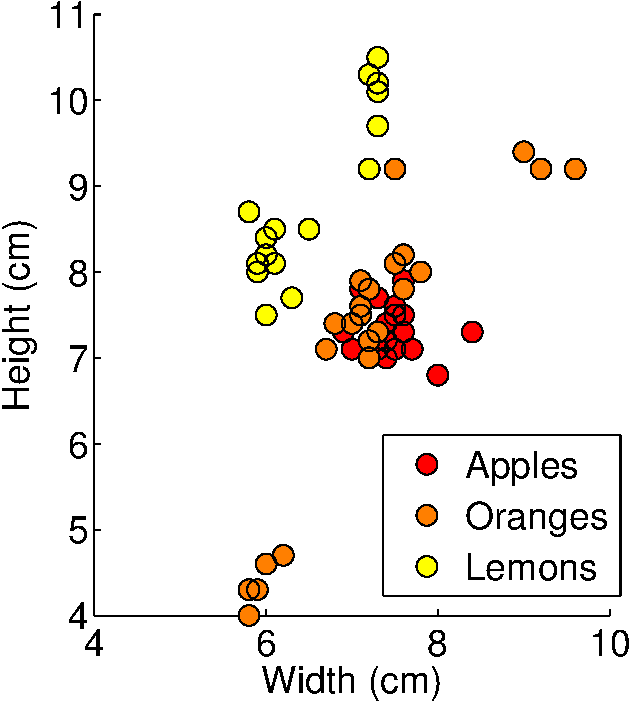
\includegraphics[width=0.5\textwidth]{fruit}
\caption{Heights and widths of apples, oranges, and lemons.  These fruit were
purchased and measured by Iain Murray:
\url{http://homepages.inf.ed.ac.uk/imurray2/teaching/oranges_and_lemons/}.}
\label{fig:fruit}
\end{figure}
\begin{problem}[Classifying Fruit, 15pts]
You should implement the following:
\begin{itemize}
\item The three-class generalization of logistic regression, also
  known as softmax regression, for these data. You will do this by implementing
  gradient descent on the negative log likelihood. You will need to find good values for the learning rate $\eta$ and regularization strength $\lambda$.
%
\item A generative classifier with Gaussian
  class-conditional densities, as in Problem~3. In particular, make
  two implementations of this, one with a shared covariance matrix
  across all of the classes, and one with a separate covariance being
  learned for each class.  Note that the staff implementation can
  switch between these two by the addition of just a few lines of
  code. In the separate covariance matrix case, the MLE for the
  covariance matrix of each class is simply the covariance of the data
  points assigned to that class, without combining them as in the
  shared case.
\end{itemize}
You may use anything in  \texttt{numpy} or \texttt{scipy}, except for \texttt{scipy.optimize}. That being said, if you happen to find a function in \texttt{numpy} or \texttt{scipy} that seems like it is doing too much for you, run it by a staff member on Piazza. In general, linear algebra and random variable functions are fine. The controller file is \texttt{problem4.py}, in which you will specify hyperparameters. The actual implementations you will write will be in \texttt{LogisticRegression.py} and \texttt{GaussianGenerativeModel.py}.


You will be given class interfaces for \texttt{GaussianGenerativeModel} and \texttt{LogisticRegression} in the distribution code,
and the code will indicate certain lines that you should not change in your final submission. Naturally, don't change these.
These classes will allow the final submissions to have consistency. There will also be a few hyperparameters that are set to
irrelevant values at the moment. You may need to modify these to get your methods to work.
The classes you implement follow the same pattern as scikit-learn, so they should be familiar to you. The distribution code currently outputs nonsense predictions just to show what the high-level interface should be, so you should completely remove the given \texttt{predict()} implementations and replace them with your implementations.

\begin{itemize}
\item The \texttt{visualize()} method for each classifier will save a plot that will show the decision boundaries. You should include these in this assignment.
\item Which classifiers model the distributions well?
\item What explains the differences?

\end{itemize}

In addition to comparing the decision boundaries of the three models visually:
\begin{itemize}

\item For logistic regression, report negative log-likelihood loss for several configurations of hyperparameters. Why are your final choices of learning rate ($\eta$) and regularization strength ($\lambda$) reasonable? Plot loss during training for the best of these configurations, with iterations on the x-axis and loss on the y-axis (one way to do this is to add a method to the LogisticRegression Class that displays loss).

\item For both Gaussian generative models, report likelihood. In the separate covariance matrix case, be sure to use the covariance matrix that matches the true class of each data point.

\end{itemize}

\end{problem}

\begin{solution}
\begin{sol}

\begin{table}[h!]
\caption{Logistic regression losses}
\begin{tabular}{llll}
$\eta$ & $\lambda$ & iterations & loss  \\
$10^{-5}$ & 0      & 140874     & 32.48 \\
$10^{-5}$ & 0.01   & 132960     & 32.88 \\
$10^{-5}$ & 0.1    & 105161     & 35.32 \\
$10^{-5}$ & 1      & 89798      & 42.49 \\
$10^{-4}$ & 0      & 14087      & 32.48 \\
$10^{-4}$ & 0.01   & 13296      & 32.88 \\
$10^{-4}$ & 0.1    & 10516      & 35.32 \\
$10^{-4}$ & 1      & 8980       & 42.49
\end{tabular}
\end{table}

The generative model with separate covariances performs the best.
All three classifiers separate out the green (lemons) well.
Logistic regression and the generative model with shared covariances struggle to separate the red (apples) and blue (oranges).
They produce linear decision boundaries and the data are not linearly separable.
The generative model with separate covariances performs better separating the red and blue,
because it can produce non-linear decision boundaries, e.g. a tight ellipse around the red region.
However, there is still one region where red and blue points overlap and separation is impossible.

We select a learning rate $\eta = 10^{-4}$, because smaller step sizes take longer to converge during gradient descent, and a larger $\eta = 10^{-3}$ does not converge.
We would need to do cross-validation on a testing set to select an appropriate regularization parameter $\lambda$, although 0, 0.01, and 0.1 all seem to give similiar decision boundaries.
Note that loss increases with regularization because we penalize larger magnitude weights more, so if we only cared about the training data $\lambda = 0$ gives the least bias.
Interestingly, higher regularization also converges slightly faster.

The generative model with separate covariances has a training loss (negative log likelihood) of 158.15, while the model with shared covariances has a loss of 208.41.
The model with separate covariances has more degrees of freedom and can better fit the data.

\begin{figure}[h!]
  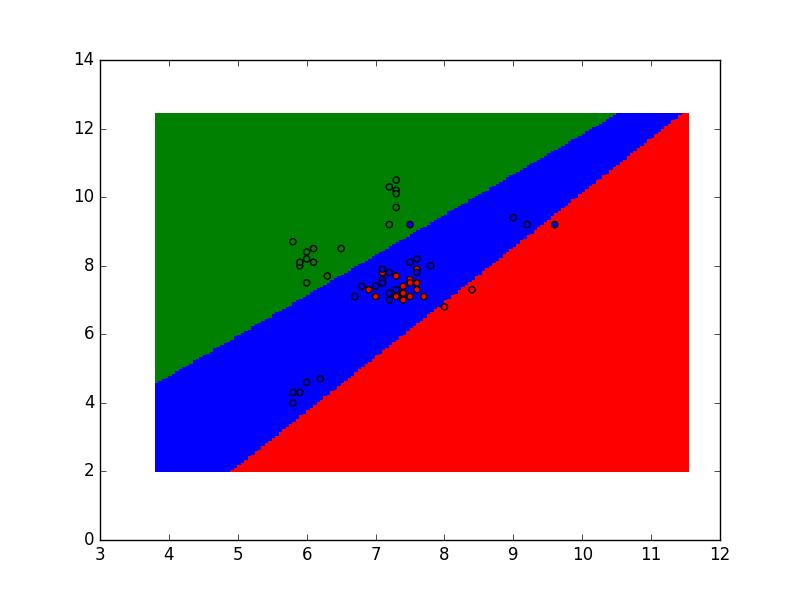
\includegraphics[width=4.5in]{logistic_regression_result.png}
  \caption{Logistic regression for $\eta = 10^{-4}$ and $\lambda = 0$.}
\end{figure}

\begin{figure}[h!]
  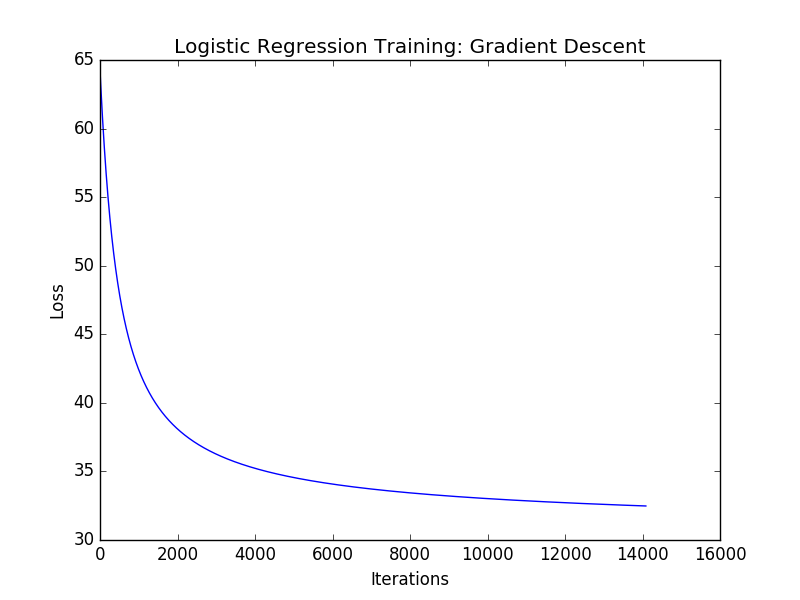
\includegraphics[width=4.5in]{logistic_regression_loss.png}
  \caption{Training loss for $\eta = 10^{-4}$ and $\lambda = 0$.}
\end{figure}

\begin{figure}[h!]
  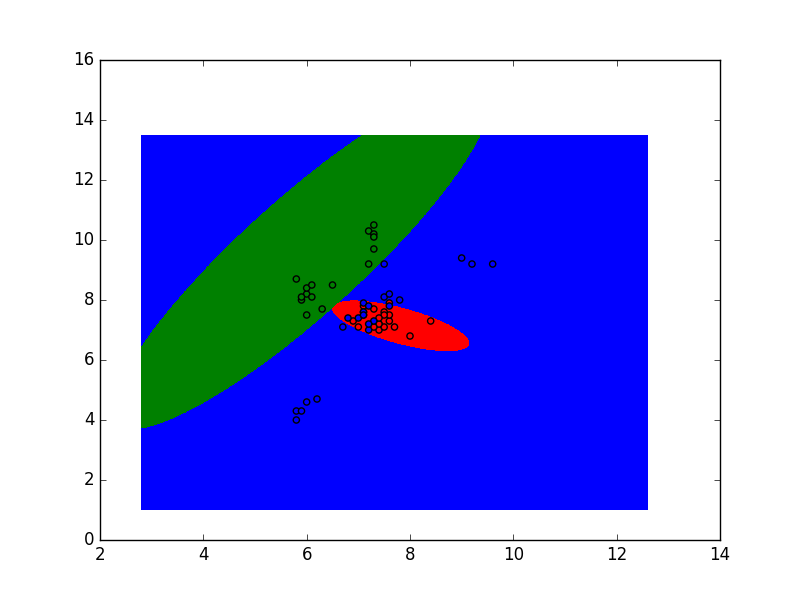
\includegraphics[width=4.5in]{generative_result_separate_covariances.png}
  \caption{Generative model with separate covariances.}
\end{figure}

\begin{figure}[h!]
  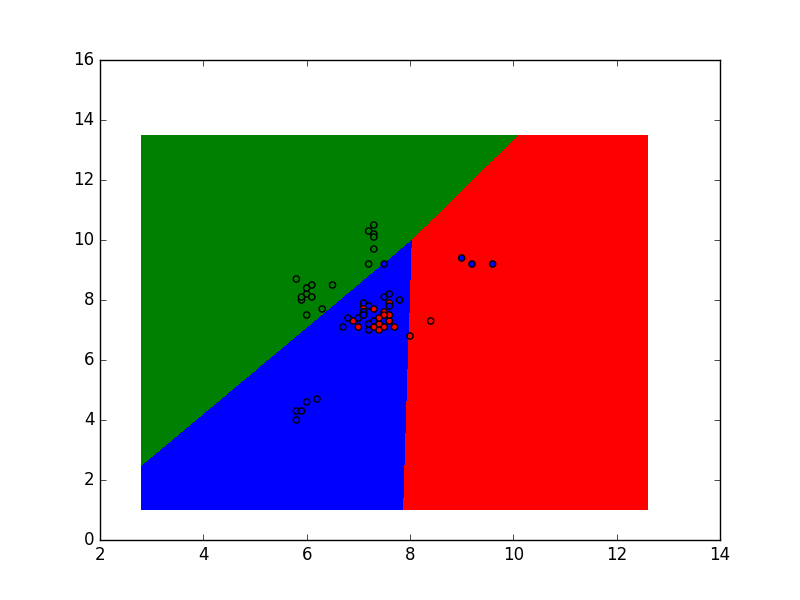
\includegraphics[width=4.5in]{generative_result_shared_covariances.png}
  \caption{Generative model with shared covariances.}
\end{figure}

\end{sol}
\end{solution}


\newpage
\subsection*{Calibration [1pt]}
Approximately how long did this homework take you to complete?
22 hours

\end{document}
